sucio.tex

% \begin{frame}[fragile]{Estudio de la heterogeneidad celular}
%   \vskip0.5em
%   Necesidad de herramientas para el estudio de la heterogeneidad celular.
%   % \Fontvi
%   \vskip-1em
%   \begin{overlayarea}{\linewidth}{1\textheight}
%   \begin{columns}
    
%     \begin{column}{0.65\textwidth}
%       \vskip-0.5em
%       \begin{alertblock}{Tradicionalmente}
%         \vskip1mm
%         A nivel de proteína mediante técnicas inmunohistoquímicas, inmunofluorescencencia y citometría de flujo. 
%       \end{alertblock}
%       \begin{alertblock}{Tecnologías de alto rendimiento}
%         \vskip1mm
%         A nivel transcriptómico mediante NGS: \textit{RNA-seq}.\\
%         \vskip1mm
%         Dos variantes:
%       \end{alertblock}
%     \end{column}

%     \begin{column}<2,3,4>{0.3\textwidth}
%       \vskip7mm
%       \begin{highlightblock}
%         \centering
%         \Fontvi{Pequeña combinación de marcadores génicos.}
%       \end{highlightblock}
%       \vskip1mm
%       \begin{highlightblock}
%         \centering
%         \Fontvi{Estatus funcional completo.}
%       \end{highlightblock}
%     \end{column}
%   \end{columns}
  
%   \vskip-1.5em

%   % Parte inferior
%   \begin{columns}
%     \begin{column}<2,3,4>{0.7\textwidth}
%       \Fontvi
%       \begin{itemize}
%         \item \textit{Bulk RNA-seq} (nivel tisular): los niveles de expresión corresponden al sumatorio de tipos celulares presentes en las muestras.
%         \vskip5mm
%         \item \textit{Single-cell RNA-seq} (nivel celular): los niveles de expresión corresponden a cada célula individual que compone la muestra.
%       \end{itemize}
%     \end{column}

%     \begin{column}{0.3\textwidth}
%       \begin{figure}
%         \centering
%         \hskip-4mm
%         \includegraphics<3,4>[width=4cm]{images/tumor_bw_arrow.png}\\
%         \hskip-4mm
%         \includegraphics<4>[width=4cm]{images/tumor_color_arrow.png}  
%       \end{figure}
      
%     \end{column}
%   \end{columns}
% \end{overlayarea}
% \end{frame}



\begin{frame}{Introducción: Clustering}
    \vskip1em
    Conocer la \alert{\textbf{estructura de las poblaciones celulares}}.
    \Fontvi
    \vskip0.5em
    \begin{columns}
      \begin{column}{0.5\textwidth}
        \begin{alertblock}{Por qué}
          \begin{itemize}
            \item Qué fenotipos hay presentes.
            \item Qué perfiles de expresión.
            \item Qué células son similares y qué celulas no.
          \end{itemize}
        \end{alertblock}
        \begin{alertblock}{Características}
          \begin{itemize}
            \item Escalable.
            \item No paraḿetrico.
            \item Alta dimensionalidad.
            \item Geometrías no estándar.
          \end{itemize}
        \end{alertblock}
      \end{column}
      \begin{column}{0.4\textwidth}
        \begin{textblock*}{5cm}(7cm,3cm)
          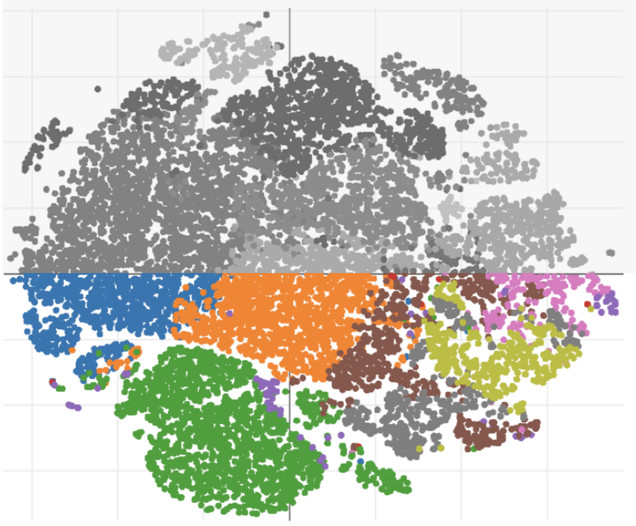
\includegraphics[scale=.5]{images/10x_mod.jpg}
        \end{textblock*}
      \end{column}
    \end{columns}
  
    \begin{center}
      \fontsize{15}{7.2}\selectfont
      \begin{itemize}
        \begin{center}
          \vskip1em
          \hskip-12mm
          \item<2>[\alert{\textbf{PhenoGraph}}]
        \end{center}
      \end{itemize}
      % \alert{\textbf{PhenoGraph}}  
    \end{center}
  \end{frame}
  
  %--------------------------------------------------------------------------%
  
  
  \section{PhenoGraph}
  
  \begin{frame}{PhenoGraph}
    \alert{Aprendizaje no supervisado:}
    Agrupa $N$ células individuales en subpoblaciones (clústers) que representan los fenotipos
    presentes en la muestra.
    \begin{itemize}
      \item Input: matriz $N$x$D$.
      \item Busca regiones densas en el espacio $D$-dimensional $\rightarrow$ grafo.
      \item Busca comunidades en el grafo.
      \item Output: index asignando cada célula a una subpoblación.
    \end{itemize}
    \vskip-0.5em
    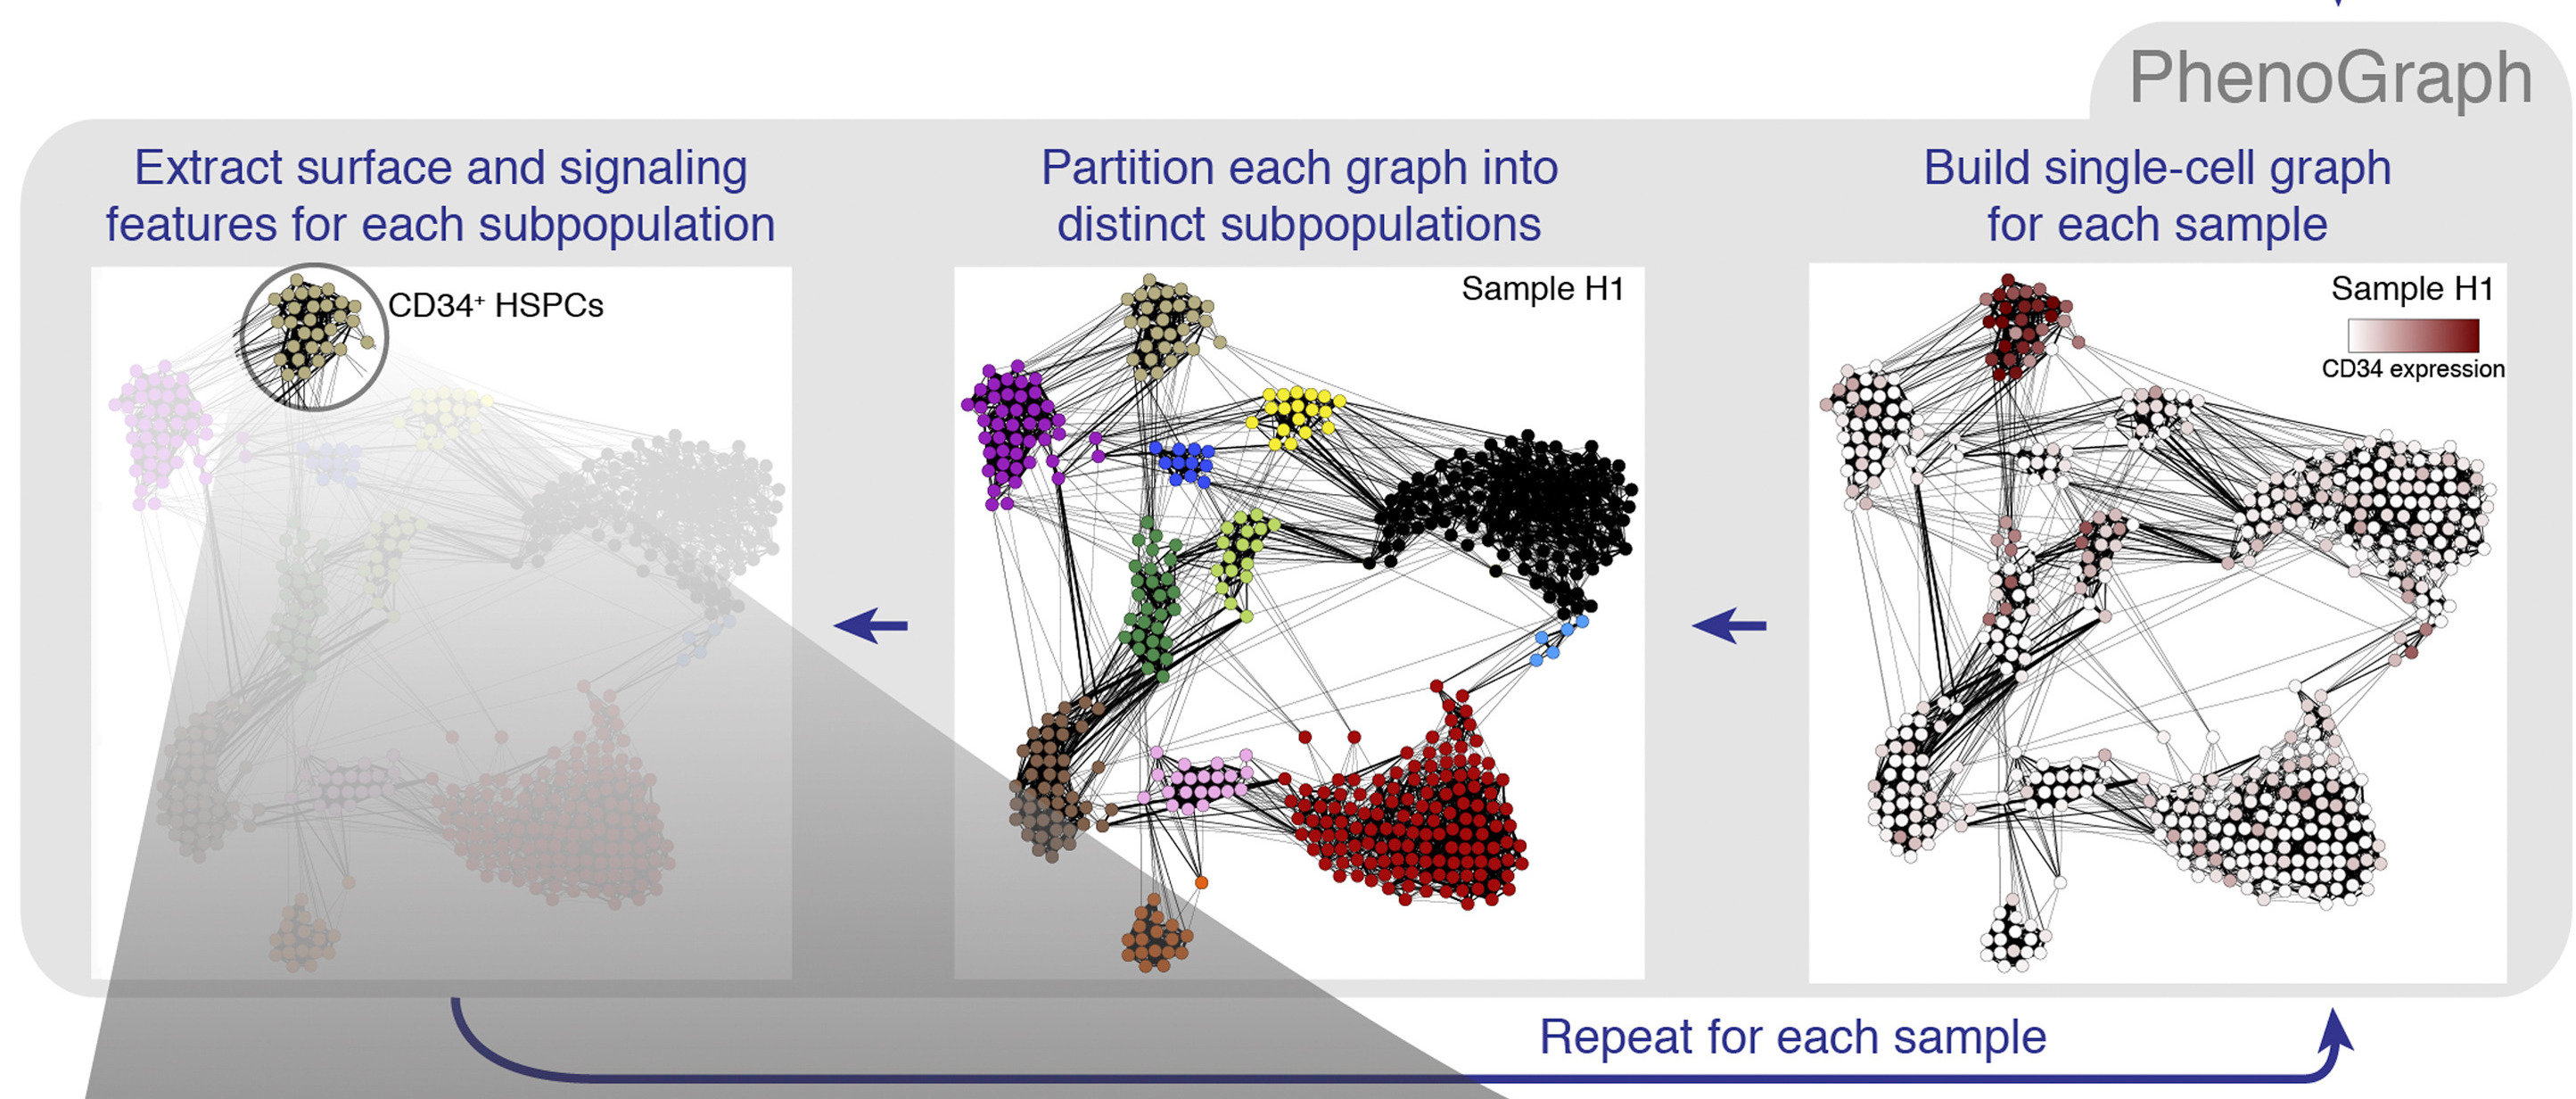
\includegraphics[scale=.72]{images/gr1_lrg_C.jpg}
  
  \end{frame}
  
  %--------------------------------------------------------------------------%
  
  \subsection{1. Construcción del grafo}
  
  \begin{frame}{Construcción del grafo: kNN}
    \vskip1em
    \begin{beamercolorbox}[sep=0.2cm,center]{coloredboxstuff}
      \textbf{Paso 1: $k$-Nearest-Neighbors}
    \end{beamercolorbox}
    \vskip-0.2cm
    \begin{itemize}
      \item $k$ vecinos más cercanos para cada célula con distancia Euclidea.
      \item Si $k$ es bajo, baja conectividad entre las poblaciones.
      \item Si $k$ es alto, resolución de poblaciones pequeñas se pierde.
      \item $N$-células con $k$-vecinos: $N$ agrupaciones.
    \end{itemize}
  
    \vskip0.5em
    \begin{columns}
      \hskip1.3em
      \begin{column}{0.5\textwidth}
        % \centering
        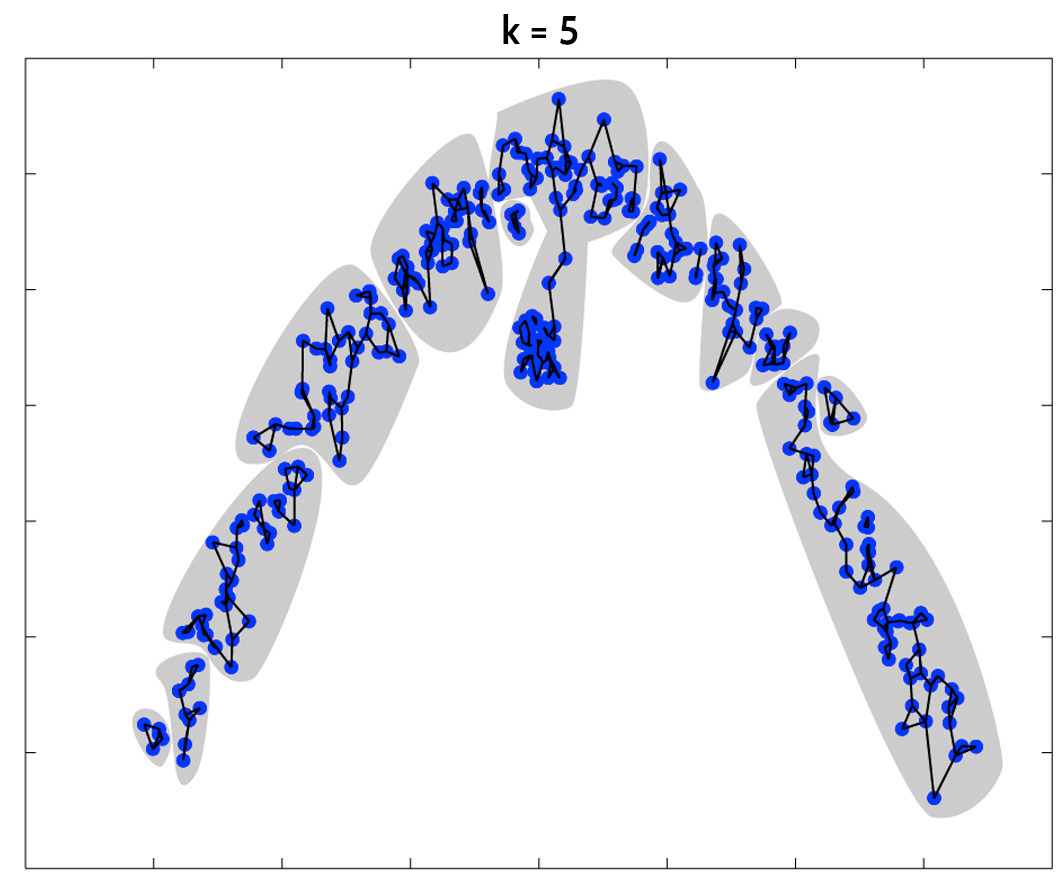
\includegraphics[scale=.9]{images/k5_knn.jpg}
      \end{column}
      \hskip-1.3em
      \begin{column}{0.5\textwidth}
        % \centering
        \vskip-0.4mm
        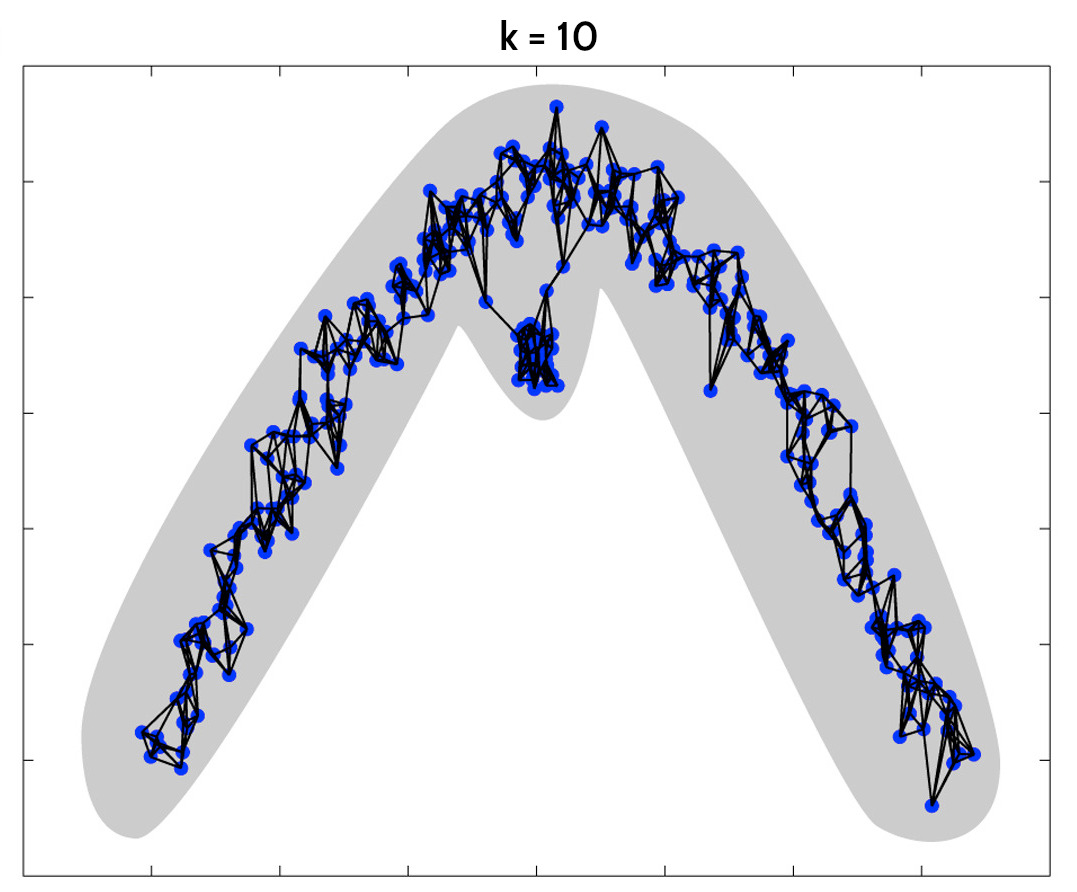
\includegraphics[scale=.9]{images/k10_knn.jpg}
      \end{column}
    \end{columns}
  \end{frame}
  
  %--------------------------------------------------------------------------%
  
  \begin{frame}{Construcción del grafo: Coeficiente de similitud de Jaccard}
    \vskip1em
    \begin{beamercolorbox}[sep=0.2cm,center]{coloredboxstuff}
      \textbf{Paso 2: Índice de Jaccard}
    \end{beamercolorbox}
    \vskip-0.2cm
    \begin{itemize}
      \item Redefinición de $k$-vecinos de cada célula definidos por $k$NN.
      \item Índice de Jaccard: similitud entre dos conjuntos.
    \end{itemize}
  
    \begin{columns}
      \begin{column}{0.5\textwidth}
        \hskip8mm
        \begin{equation*}
          W_{i, j} = \frac{|v(i) \cap v(j)|}{|v(i) \cup v(j)|}
        \end{equation*}
      \end{column}
      \begin{column}{0.5\textwidth}
        \vskip0.2em
        \hbox{\hspace{-0.5em}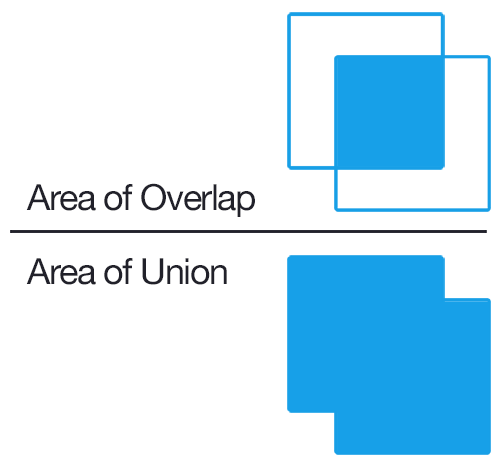
\includegraphics[scale=.2]{images/equation_jaccard_1.png}}
      \end{column}
    \end{columns}
    % \metroset{block=fill}
    \begin{textblock*}{5cm}(5.45cm,4.63cm)
      
\includegraphics[scale=0.04]{images/equal.jpg}
    \end{textblock*}
    \begin{alertblock}{Intuitivamente}
      \begin{itemize}
        \item La similitud entre células será máxima cuando sus $k$-vecinos son los
              mismos $\rightarrow$ mismo fenotipo.
        \item Similitud decaerá entre células que compartan menos vecinos conectados
              $\rightarrow$ distinto fenotipo.
      \end{itemize}
    \end{alertblock}
  \end{frame}
  
  %--------------------------------------------------------------------------%
  
  \begin{frame}{Construcción del grafo: Coeficiente de similitud de Jaccard}
    % \metroset{block=fill}
    % \vskip-1em
    \begin{alertblock}{Resultado}
      \vskip0.20em
      Grafo ponderado con pesos basados en el número de vecinos que comparten.
    \end{alertblock}
  
    \begin{alertblock}{Qué conseguimos}
      \begin{itemize}
        \item Incorporamos la estructura de la distribución de los datos al grafo a
              través de los pesos.
        \item Estructura compacta y rica en información que captura la similitud entre células.
      \end{itemize}
    \end{alertblock}
    \begin{columns}
      \begin{column}{0.6\textwidth}
        \vskip-5em
        \hskip-3cm
        \begin{itemize}
          \item Se refuerzan ejes en zonas densas.
          \item Se penalizan ejes en zonas dispersas.
          \item Poblaciones raras son mejor resueltas.
          \item Outliers tienden a ser excluídos.
        \end{itemize}
      \end{column}
      \begin{column}{0.46\textwidth}
        \vskip-0.5em
        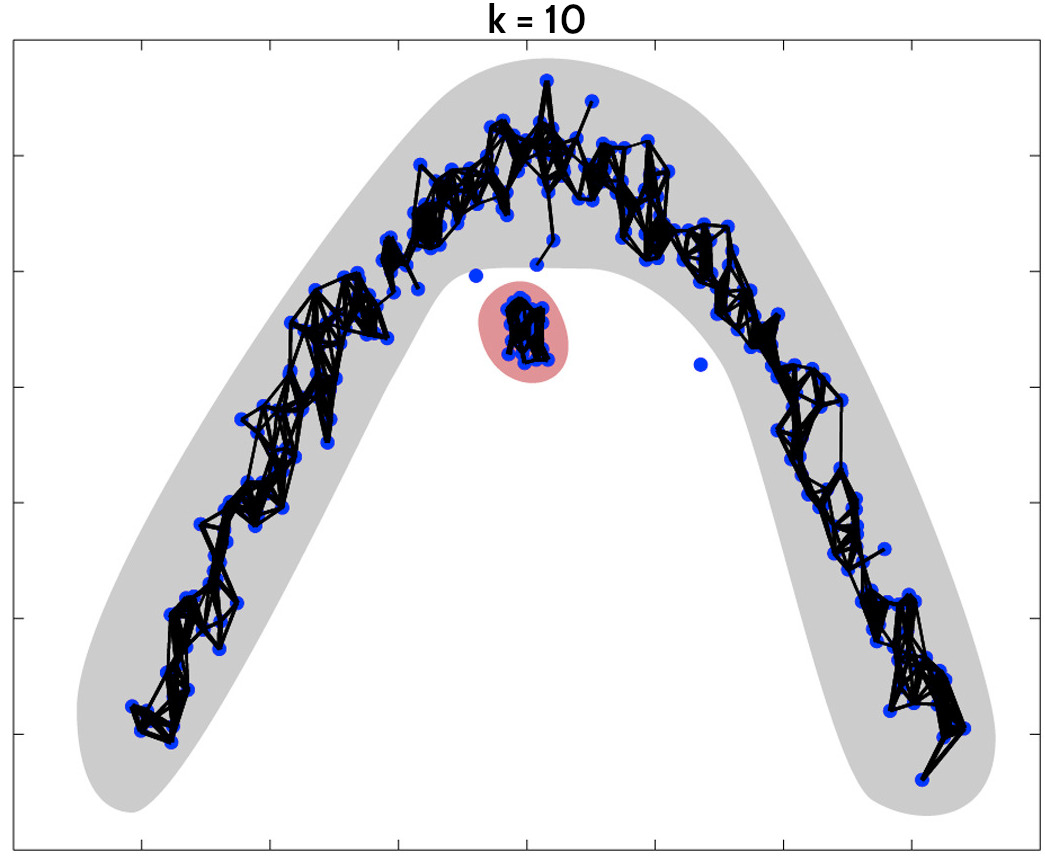
\includegraphics[scale=0.9]{images/figs1_lrg_D.jpg}
      \end{column}
    \end{columns}
  \end{frame}
  
  
  \begin{frame}{Partición del grafo en comunidades}
    \vskip0.2em
    \begin{alertblock}{Comunidad}
      \vskip0.5mm
      Presencia de grupos de nodos que están
      más densamente conectados entre sí que con otros nodos.
    \end{alertblock}
  
    \begin{columns}
      \begin{column}{0.4\textwidth}
        \vskip0.3cm
        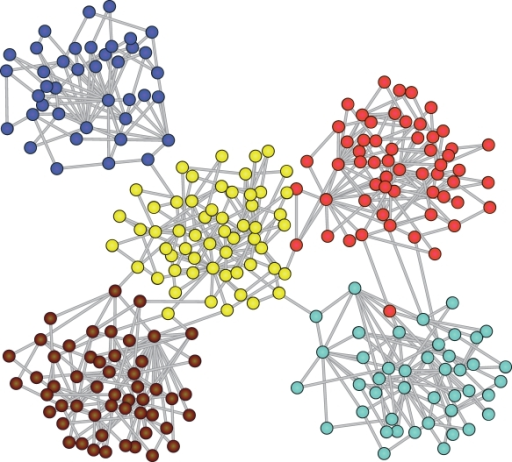
\includegraphics[scale=0.29]{images/community_graph_2.png}
      \end{column}
      \begin{column}{0.6\textwidth}
        \vspace{-3em}
        \begin{itemize}
          \item Los grafos resultantes tienen esta propiedad por cómo se han construido y
                por el tipo de datos de los que proceden.
          \item Las comunidades representan células fenotípicamente similares.
        \end{itemize}
      \end{column}
    \end{columns}
    \vskip0.5em
    \begin{beamercolorbox}[sep=0.2cm,center]{coloredboxstuff}
      Cómo encontramos las comunidades.
    \end{beamercolorbox}
    \begin{beamercolorbox}[sep=0.2cm,center]{coloredboxstuff}
      Cómo dividimos el grafo de forma óptima.
    \end{beamercolorbox}
  \end{frame}
  
  
  \subsection{2. Partición del grafo en comunidades}
  
  \begin{frame}{Partición del grafo en comunidades: Modularidad}
    \begin{overlayarea}{\linewidth}{1\textheight}
      % \vskip0.2em
      \begin{alertblock}{Modularidad ($Q$)}
        \vskip0.5mm
        Medida de la calidad de una división particular de una red.
        Puede ser utilizada como función objetivo a maximizar por
        los algoritmos de detección de comunidades.
      \end{alertblock}
  
      % \vskip-1em
      \only<1>{
        \begin{equation*}
          Q = \frac{1}{2m} \sum_{i,j}\left[W_{i,j} - \frac{s_i s_j}{2m}\right]\delta(c_i,c_j)
        \end{equation*}
        % \vskip-1em
      }
  
      \only<2>{
        \vskip1em
        \centering
        \hspace{1.6em}
        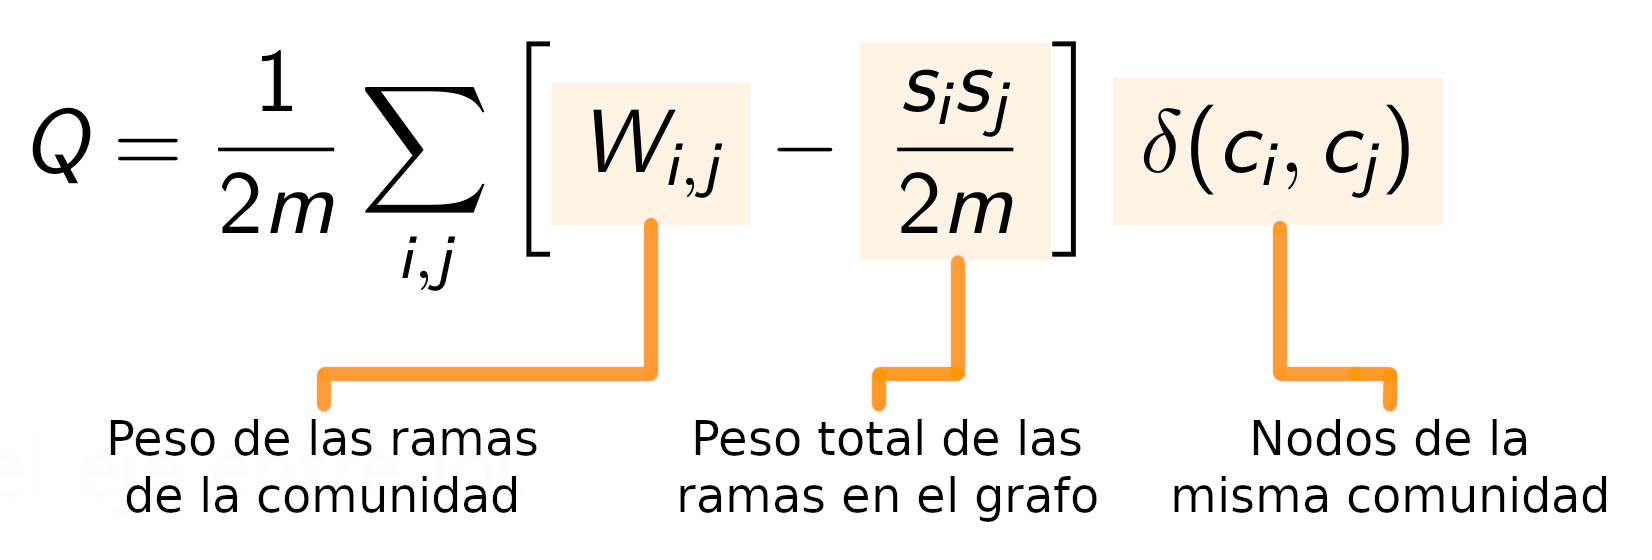
\includegraphics[scale=0.13]{images/equation_good.png}
      }
      \only<1>{
        \vskip0.5em
        \begin{itemize}
          \item $W_{i,j}$: peso del eje entre los nodos $i$ y $j$.
          \item $s_i$: suma de los pesos de los ejes que involucran al nodo $i$.
          \item $c_i$: asignación de la comunidad para el nodo $i$.
          \item $\delta(u,v)$: función delta de Kronecker: 1 si $u = v$, 0 si $u \neq v$.
          \item $m = \frac{1}{2} \sum W_{i,j}$: peso total de la red.
        \end{itemize}
      }
      \only<2>{
        \begin{alertblock}{Intuitivamente}
          \begin{itemize}
            \item Solo se calcula para pares de nodos de la misma comunidad.
            \item Cuando $W_{i,j}$ es mayor, la modularidad es más alta.
            \item Cuando $\frac{s_i s_j}{2m}$ es mayor, la modularidad baja.
          \end{itemize}
        \end{alertblock}
      }
    \end{overlayarea}
  \end{frame}
  
  \begin{frame}{Partición del grafo en comunidades: Modularidad}
    \vskip1em
    \hbox{\hspace{-0.5em}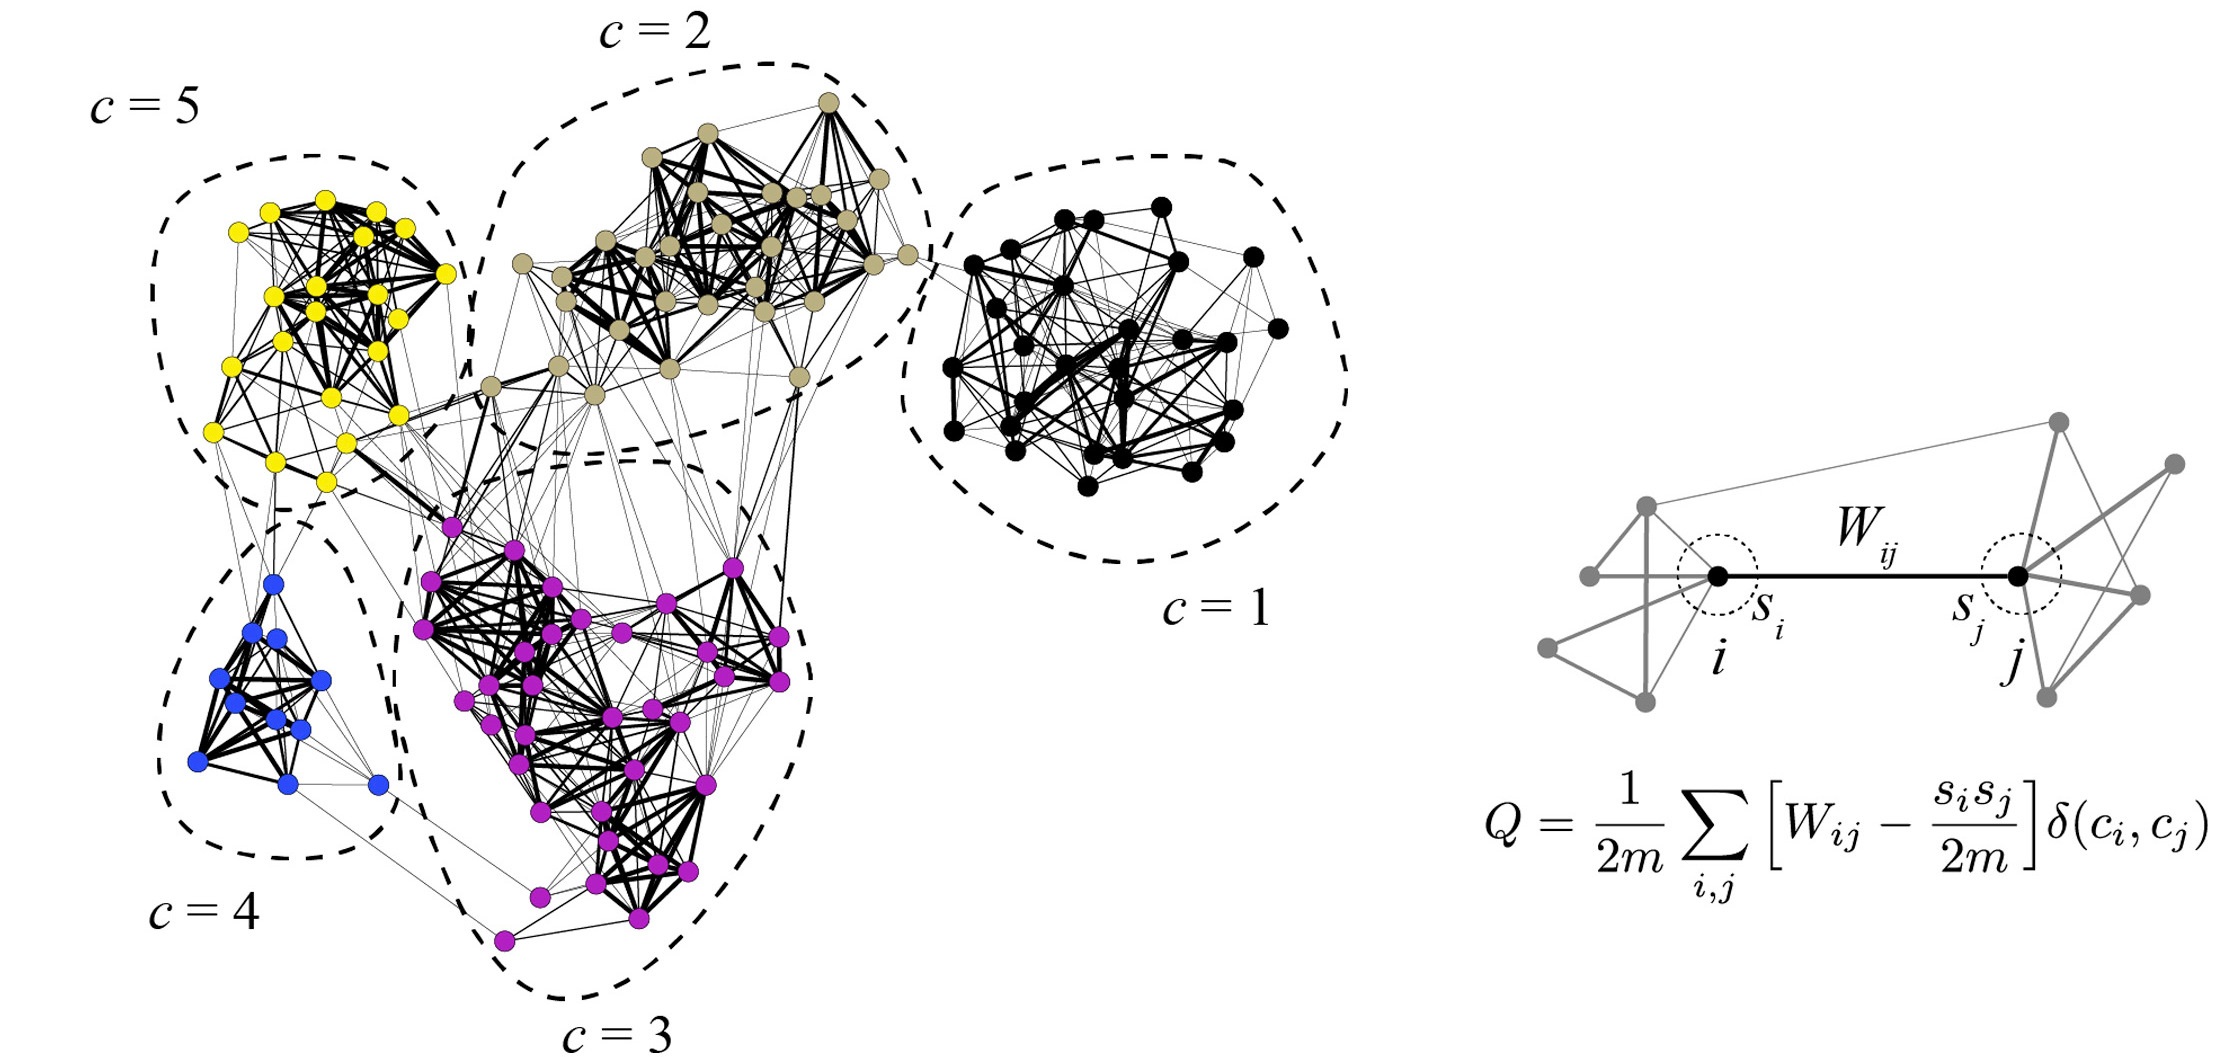
\includegraphics[scale=0.95]{images/louvain_example.jpg}}
    \vskip1em
    \begin{beamercolorbox}[sep=0.2cm,center]{coloredboxstuff}
      Búsqueda óptima: Problema de optimización combinatorial \textbf{NP-completo}.
    \end{beamercolorbox}
    \begin{beamercolorbox}[sep=0.2cm,center]{coloredboxstuff}
      Necesitamos algoritmos heurísitcos: \textbf{Método de Louvain}.
    \end{beamercolorbox}
  \end{frame}
  
  
  \begin{frame}{Partición del grafo en comunidades: Método de Louvain}
    % \vskip-9em
    \vskip0.2em
    Aproximación heurística con dos fases repetidas iterativamente:
    \Fonteight
    \begin{alertblock}{Primera fase}
      \begin{enumerate}[<+-| alert@+>]
        \item Se asigna una comunidad a cada nodo ($N$ comunidades).
        \item Cada nodo $i$ se asgina a la de cada vecino $j$ y
              se calcula $\Delta Q$.
        \item Si $\Delta Q$ resultante es positiva, se asigna $i$ a dicha comunidad.
      \end{enumerate}
    \end{alertblock}
    \begin{alertblock}{Segunda fase}<4->
      \vskip-0.2mm
      \begin{enumerate}[<+-| alert@+>]
        \item Se construye una nueva red con las comunidades obtenidas anteriormente
              como nodos.
        \item Los pesos se computan como la suma de los pesos de cada comunidad.
  
      \end{enumerate}
    \end{alertblock}
    \centering
    \vskip-1em
    % \begin{textblock*}{1cm}(3.3cm,5.8cm)
    % 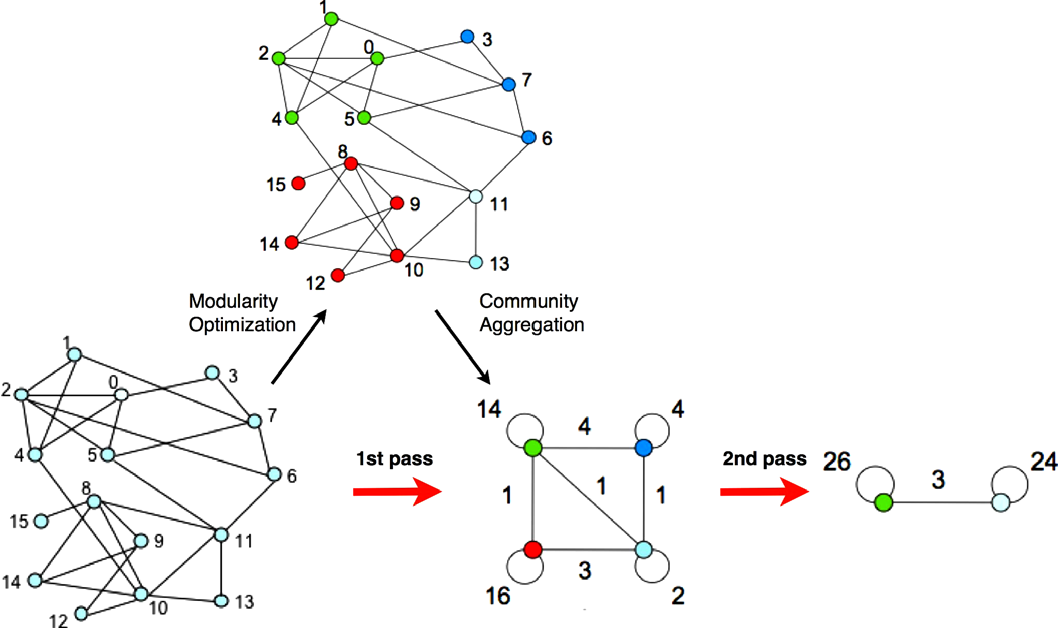
\includegraphics[scale=0.18]{images/louvine_method.png}
    \includegraphics<1,2,3>[scale=0.18]{images/louvine_method_3.png}
    \includegraphics<4,5>[scale=0.18]{images/louvine_method_4.png}
    \includegraphics<6>[scale=0.18]{images/louvine_method_5.png}
    % \end{textblock*}
  
  \end{frame}
  
  
  
  \begin{frame}{Pseudocódigo}
    \vskip-0.5em
    \textbf{Input:} data set of single-cell measurements $X = \{x1, .., xN\}$\\
    \textbf{Output:} subpopulation index assigning each cell in X to one of M groups\\
    \vskip2em
    \begin{beamercolorbox}[sep=0.2cm]{coloredboxstuff}
      \Fontvi
      \textbf{Inicialización:}\\
      \hspace{0.5cm}\texttt{for each cell $x_i$}\\
      \hspace{1.5cm}\texttt{find the indices ν(i) of the k nearest cells}\\
      \textbf{Construcción del grafo:}\\
      \hspace{0.5cm}\texttt{set of vertices $V = \{v_1 , ..., v_N\}$ to each cell in $X$}\\
      \hspace{0.5cm}\texttt{set of edges $E = \{\}$}\\
      \hspace{0.5cm}\texttt{for each pair of cells $x_i$ and $x_j$}\\
      \hspace{1.5cm}\texttt{compute $W_{ij}$}\\
      \hspace{1.5cm}\texttt{if $W_{ij} > 0$, add $e_{ij}$ = $W_{ij}$ to E}\\
      \hspace{0.5cm}\texttt{return $G = (V, E)$}\\
      \textbf{Detección de comunidades:}\\
      \hspace{0.5cm}\texttt{for t in \{1, ..., 100\}}\\
      \hspace{1.5cm}\texttt{decompose $G$ into $C_t$ by Louvain Method}\\
      \hspace{1.5cm}\texttt{determine best $C_t$ by maximum $Q$}\\
      \hspace{0.5cm}\texttt{return $C = C_t$}
    \end{beamercolorbox}
  \end{frame}
  
  
  
  \begin{frame}{Validación en células inmunes de adulto sano}
    \begin{overlayarea}{\linewidth}{1\textheight}
      \vskip1em
      \begin{itemize}
        \item Datos públicos: 30.000 células de médula ósea asignadas manualmente
              mediante técnicas estándar.
        \item Mayor precisión y escalabilidad que otros métodos.
        \item Robusto con diferentes parámetros.
      \end{itemize}
      \vskip1.5em
      \centering
      \includegraphics<1>[scale=0.7]{images/gr2_lrg_A.jpg}
      \vskip-1em
      \includegraphics<2>[scale=0.7]{images/histogram_performance.jpg}
      \includegraphics<3>[scale=0.8]{images/computation_time_comparison.jpg}
    \end{overlayarea}
  \end{frame}
  
  
  
  \section{Resultados}
  
  \begin{frame}{Resultados: Datos}
    \begin{figure}
      \centering
      % \hskip-1em
      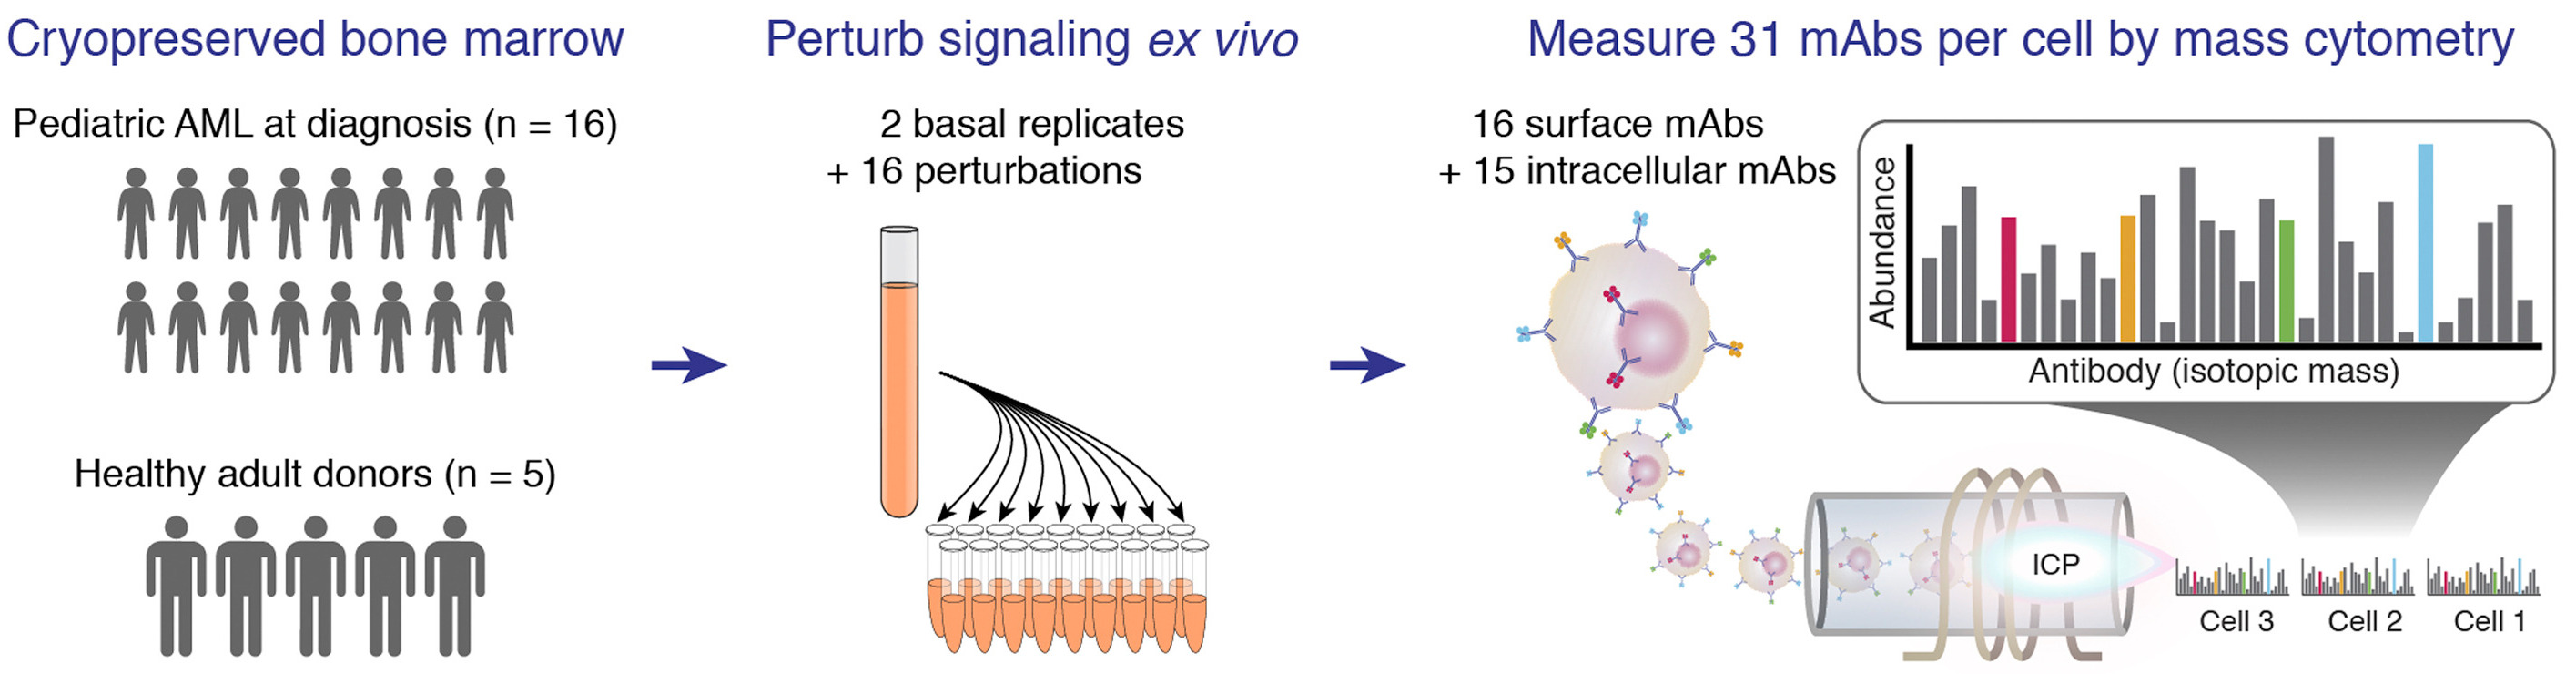
\includegraphics[scale=0.75]{images/gr1_lrg_A.jpg}
    \end{figure}
    \begin{itemize}
      \item \textbf{21 individuos:} 16 pacientes con AML, 5 adultos donantes sanos.
      \item \textbf{31 dimensiones:} \alert{16 marcadores de superficie más informativos} y 14
            sondas contra proteínas importantes en señalización intracelular.
    \end{itemize}
  \end{frame}
  
  
  \begin{frame}{Resultados: PhenoGraph sobre set de datos AML}
    \begin{itemize}
      \item PhenoGraph sobre la cohorte de pacientes AML y donantes sanos ($k$ = 50).
      \item 28 subpoblaciones / muestra.
    \end{itemize}
    \centering
    \vskip-0.5em
    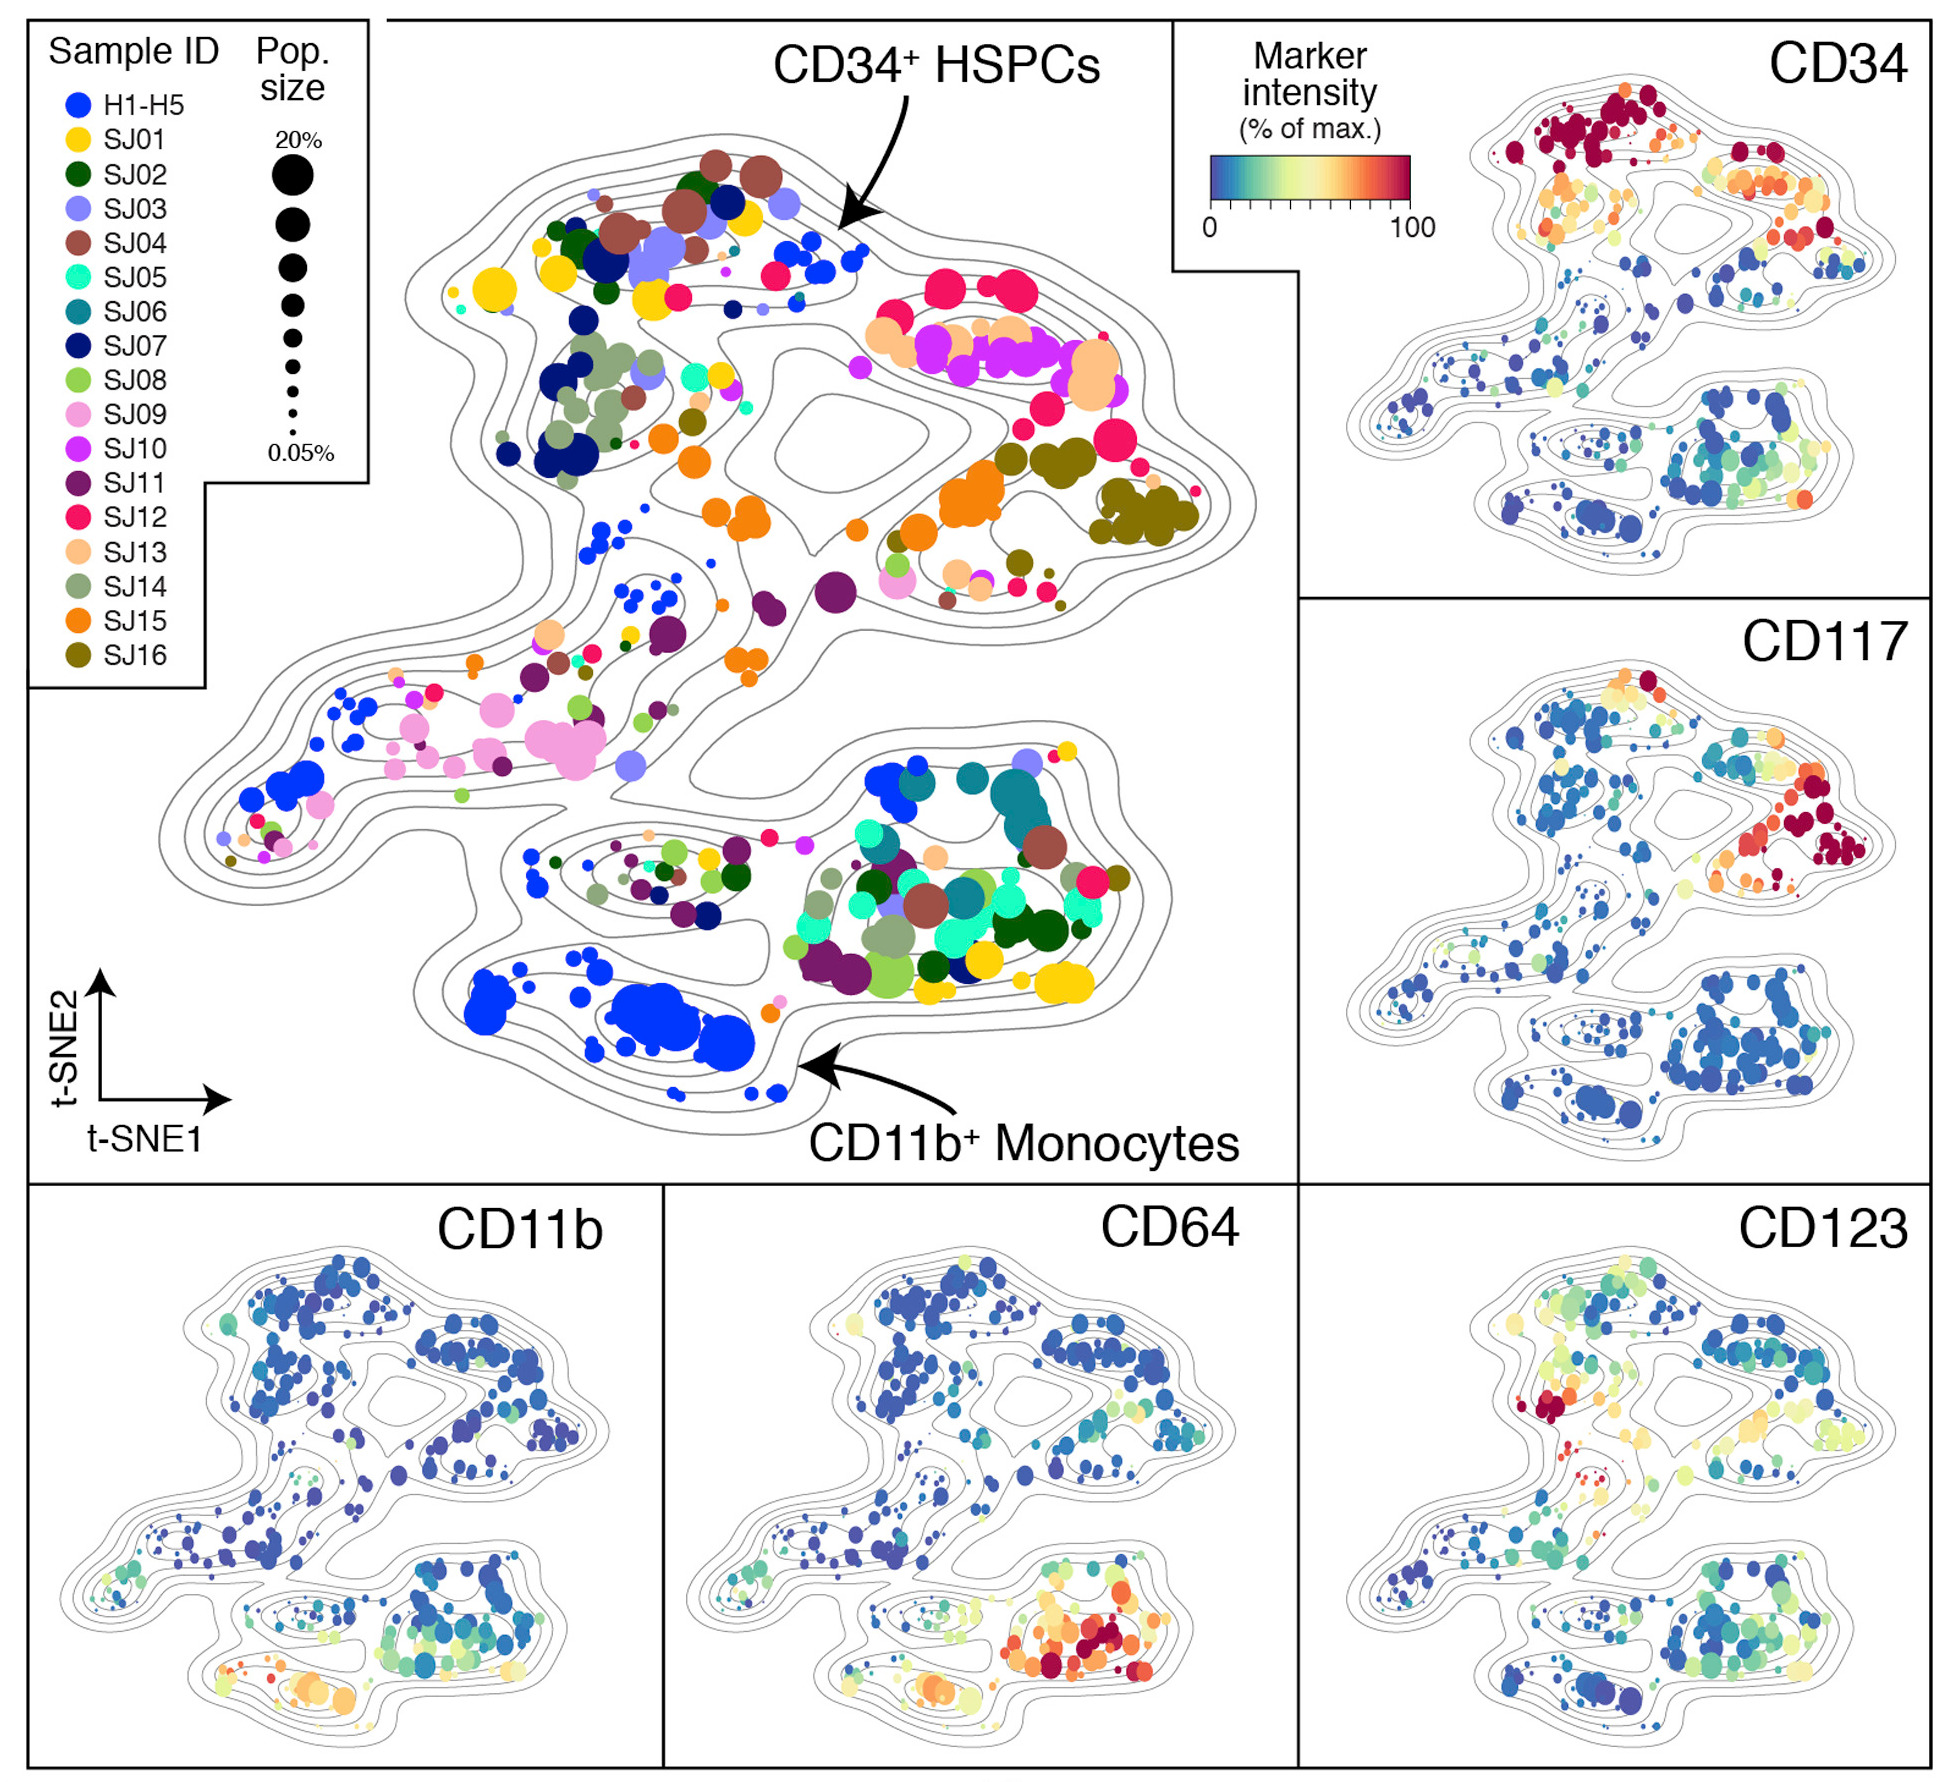
\includegraphics[scale=0.75]{images/patients_markers.jpg}
  \end{frame}
  
  
  
  \begin{frame}{Resultados: PhenoGraph sobre subpoblaciones AML}
    \begin{itemize}
      \item PhenoGraph sobre subpoblaciones AML ($k$ = 15).
      \item Cada subpoblación definida por centroides: matriz 425 x 16.
    \end{itemize}
    \centering
    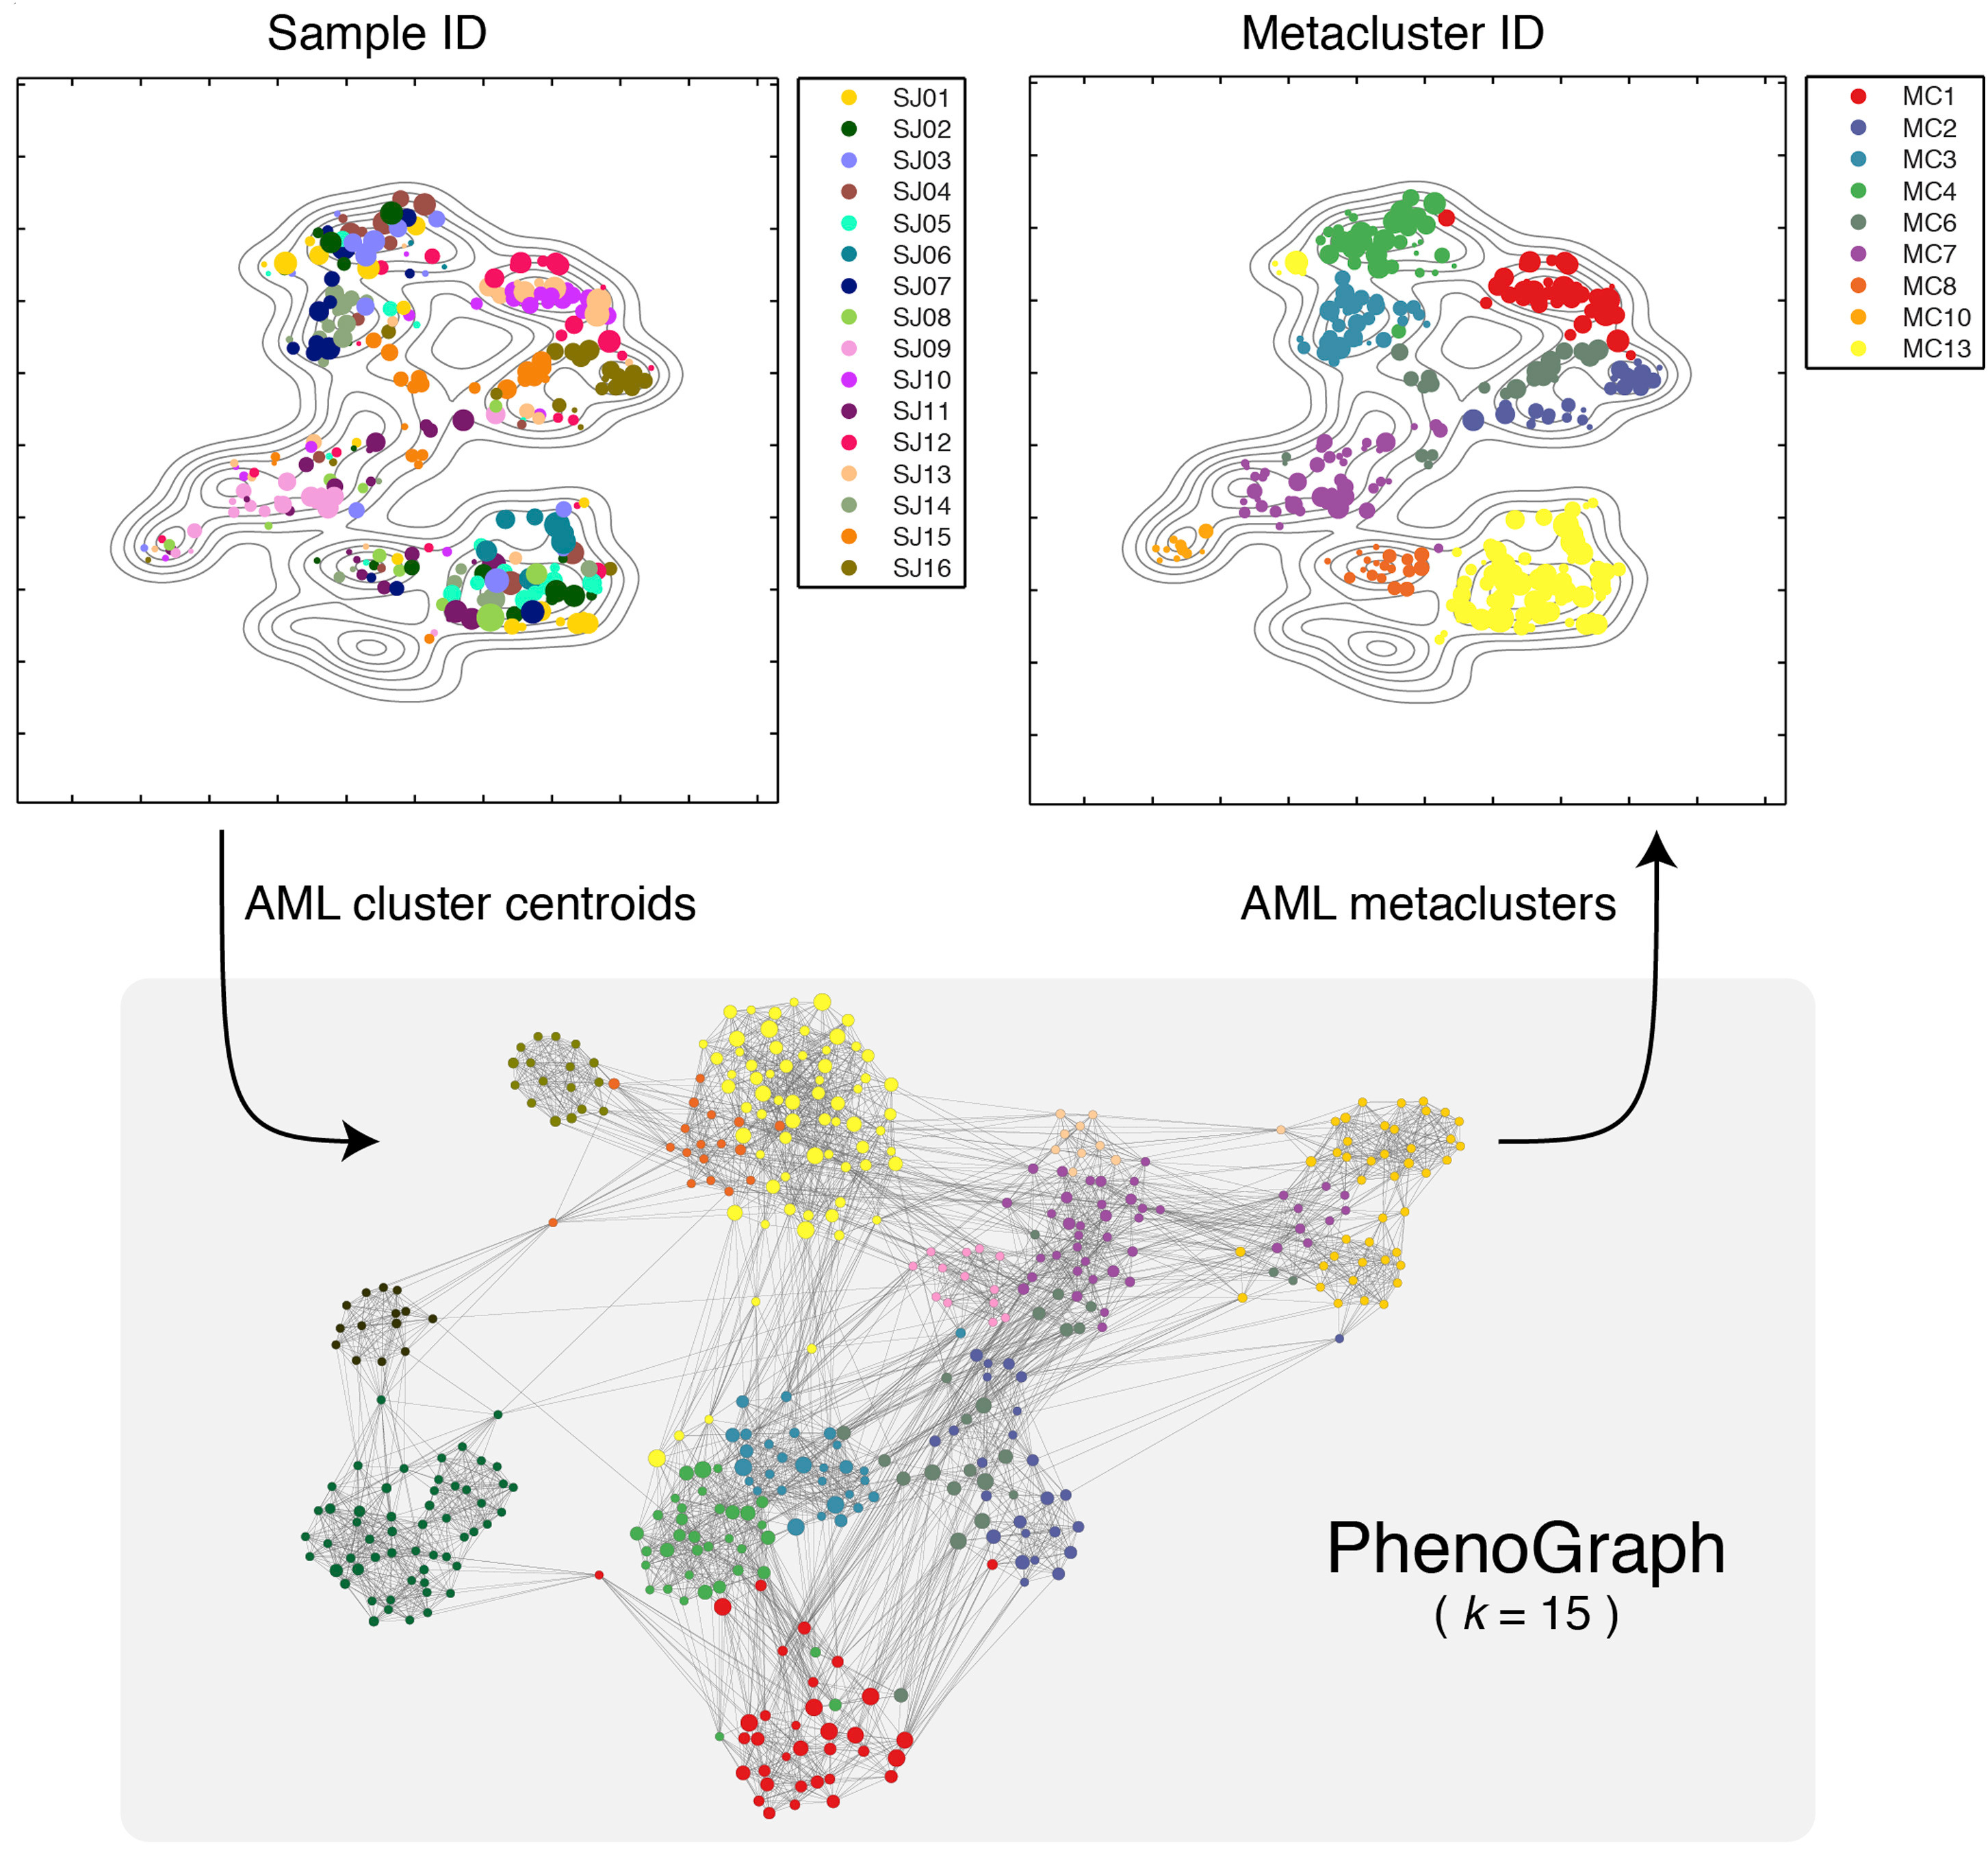
\includegraphics[scale=0.52]{images/AML_subpoblations.jpg}
  \end{frame}
  
  
  \begin{frame}{Resultados: Cross-validación}
    \begin{alertblock}{Resampleo de subpoblaciones AML}
      \Fontvi
      \begin{itemize}
        \item 16 repeticiones aleatorias de todos los datos.
        \item 1 paciente fuera: 16 sets de datos.
        \item 2 pacientes fuera: 120 sets de datos.
      \end{itemize}
    \end{alertblock}
    \vskip-0.5em
    \centering
    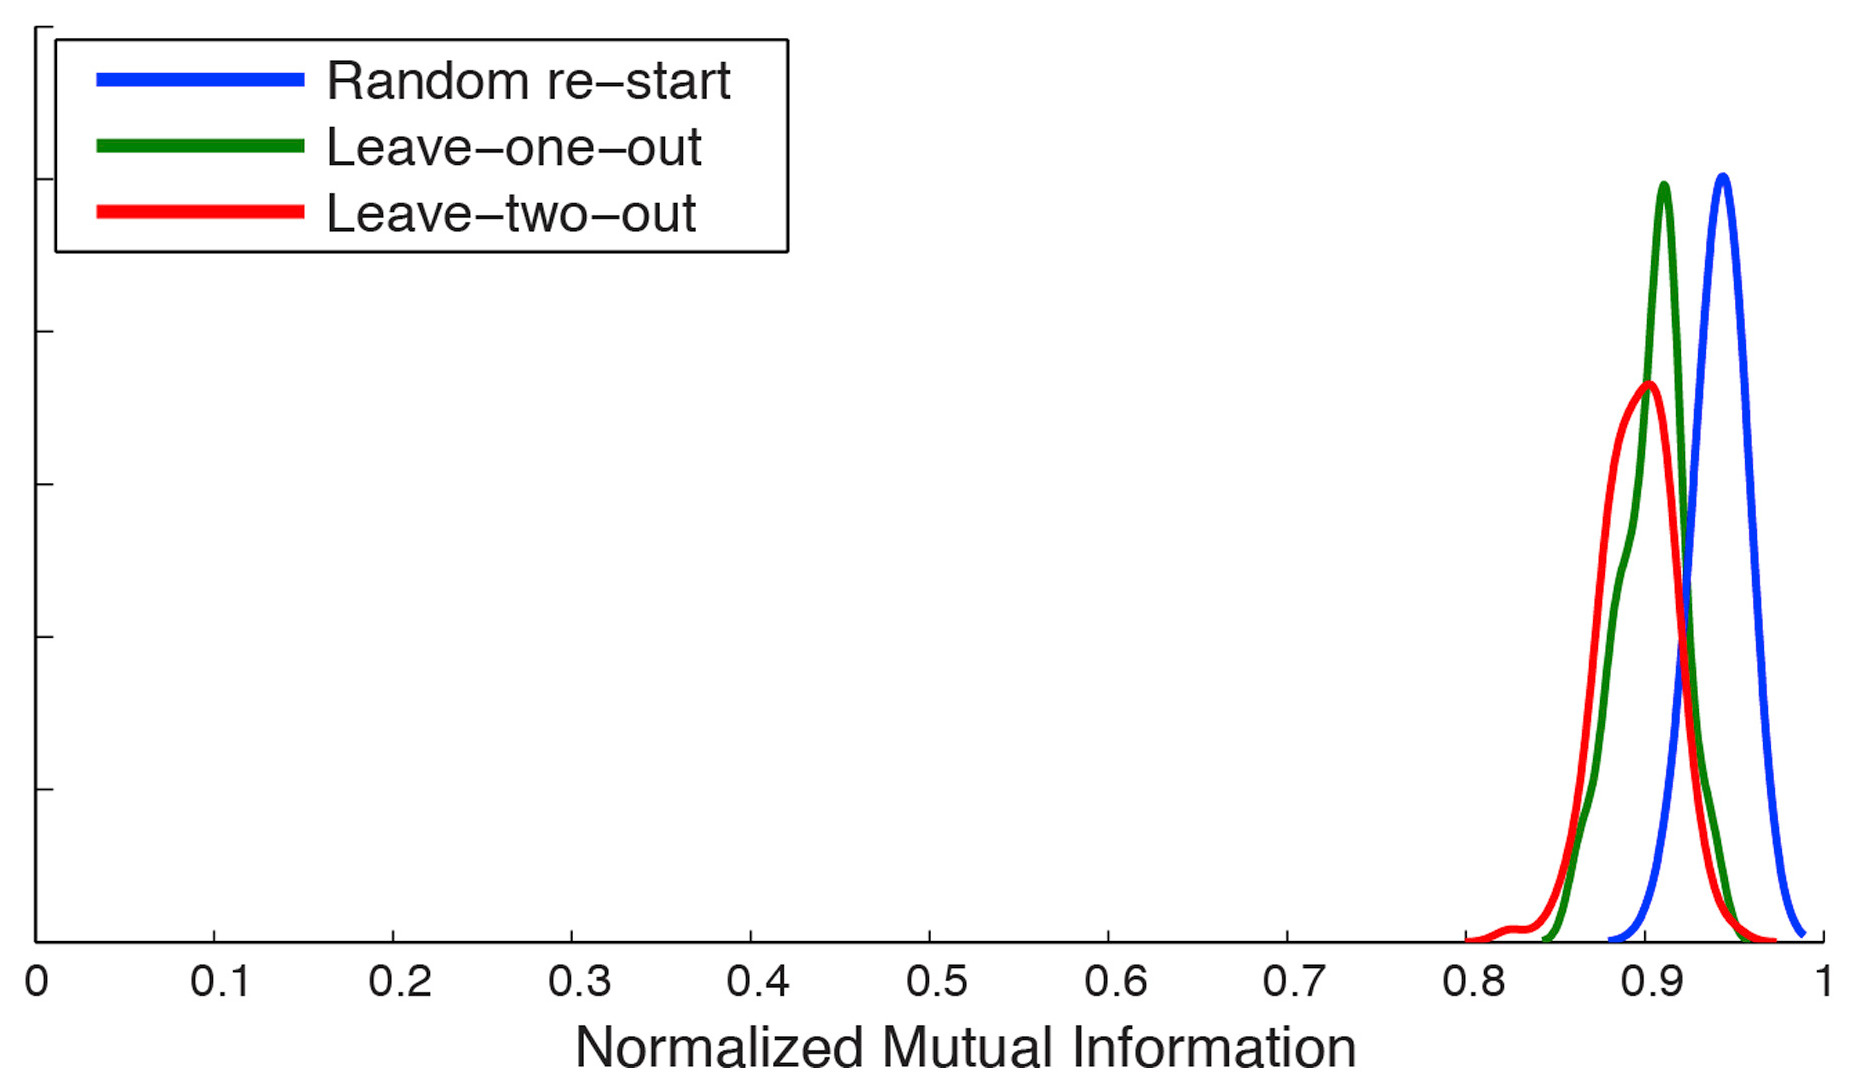
\includegraphics[scale=0.8]{images/NMI_comparison.jpg}
    \vskip0.5em
    \begin{beamercolorbox}[sep=0.2cm,center]{coloredboxstuff}
      Metaclústeres AML son robustos frente a cambios en el dataset.
    \end{beamercolorbox}
  \end{frame}
  
  
  \section{Otros métodos}
  
  \begin{frame}{Comparación con otros métodos}
    % \begin{alertblock}{Papers}
    %   % \Fontvi
    %   \begin{itemize}
    %     \item A comparison framework and guideline of clustering methods
    %     for mass cytometry data.
    %     \item Comparison of clustering methods for high‐dimensional 
    %     single‐cell flow and mass cytometry data.
    %   \end{itemize}
    % \end{alertblock}
  
    \makebox(328,90)[rt]{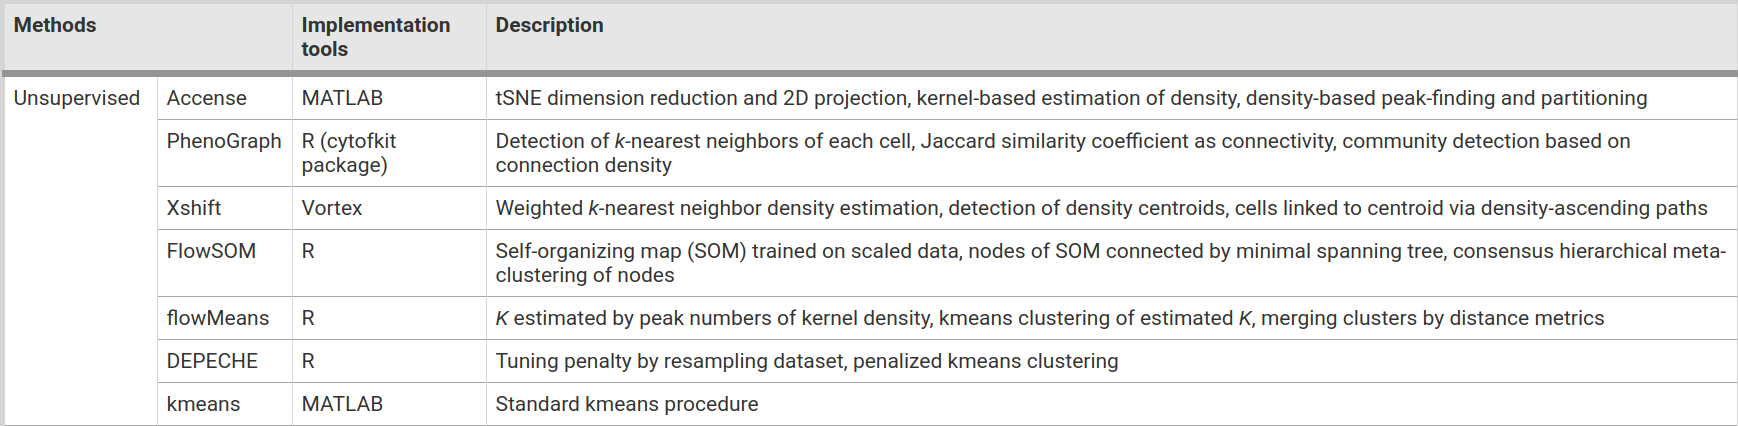
\includegraphics[scale=0.2]{images/table_methods.png}}
  
  
  
    \begin{alertblock}{Conclusiones}
      \begin{itemize}
        \item Robusto frente a cambio de parámetros y remuestreo.
        \item Preciso y escalable.
        \item Primeras posiciones junto a FlowSOM, flowMeans y DEPECHE.
      \end{itemize}
    \end{alertblock}
    \begin{alertblock}{Implementación}
      \vskip0.25em
      MATLAB, Python, R, paquetes de análisis scRNAseq (Seurat).
    \end{alertblock}
  
  \end{frame}
  
  